\documentclass[output=paper]{LSP/langsci} 
\author{Hannah Sarvasy\affiliation{MARCS Institute, Western Sydney University}}
\title{Short, finite and one-sided bridges in Logoori}

\abstract{The Luyia Bantu language Logoori shows a genre-based split in bridging construction distribution. Examination of a small corpus of Logoori texts of various genres told by diverse speakers shows that recapitulative linkage is limited to the genre in which actions are most central: procedural texts. In descriptive texts, where concepts rather than actions are topical, recapitulation occurs in the vessel of NPs, not verbs. Both types of recapitulation are largely absent from narratives. In Logoori recapitulative linkage, the predicate in the bridging clause uniformly takes the Immediate Perfect inflection, meaning ``X having just Ved''. The semantics of this inflection entail that bridging constructions cement a tight sequential relationship between the action described in the reference clause and the clause after the bridging clause. But even within the procedural text genre, recapitulative linkage is unevenly distributed and is apparently replaceable: one speaker uses the Immediate Perfect within a procedural text to effect the same sequential relationship as recapitulative linkage, but without lexical repetition. The intra-genre uneven distribution of bridging constructions, and their absence from narratives, point to their non-essentiality to Logoori discourse coherence.}
\maketitle
%-------------------------

\begin{document}
\label{ch:3}
\section{Introduction}
\label{Saintro}
\ili{Logoori} is a northeastern \ili{Bantu} language spoken in Kenya, part of the Luyia language group \citep{Mould1981}. The Luyia languages are highly of-a-piece lexically and grammatically, but no grammar of any one language exists. \ili{Logoori} is an under-described variety. Published work on the language includes a short pedagogical grammar published by the Church Missionary Society \citep{Appleby1961} and a Master’s thesis on \ili{Logoori} tone \citep{Leung1991}. Michael Diercks commissioned a corpus of \ili{Logoori} oral narratives and songs; these recordings were transcribed by \ili{Logoori} speakers in Kenya. In 2014--2015, the target language of the UCLA graduate Field Methods course, taught by the author, was \ili{Logoori}; speaker Mwabeni Indire served as consultant for the course. 

\ili{Logoori} is far from monolithic, with a high degree of dialect mixing. \ili{Logoori} phonology is distinguished by a seven-vowel inventory, multiple place distinctions for nasals, including a dental nasal, and for some speakers, an unusual interdental glide [j̪], (equivalent to [j] for other speakers). Although \ili{Logoori} is tonal, like other Luyia languages, tone does not have a high functional load. It plays no role to my knowledge in lexical distinction for nouns, or for basic grammatical distinctions in verbs such as \isi{TAM}, which are mostly marked through morphology, as in other Luyia languages (e.g.,  \citealt{Marlo2008}). Tone will be unmarked in this chapter because a full tonal analysis of \ili{Logoori} is still pending. The orthography used here is a practical orthography related to the analyses of \citet{Leung1991} and the UCLA Field Methods cohort. It differs from the orthography used by speakers in adding two vowel symbols: 〈ɛ〉 and 〈ɔ〉. \ili{Logoori} speakers use a practical orthography in which both front-high and front-mid vowels are represented with 〈i〉, but a third, lower front vowel with 〈e〉. They use 〈u〉 to represent both back-high and back-mid vowels, but 〈o〉 for a third, lower back vowel. These are distinguished in the orthography used here, so that the three front vowels are represented as: 〈i〉, 〈e〉, and 〈ɛ〉, and the three back vowels as: 〈u〉, 〈o〉, and 〈ɔ〉. Further, long vowels are represented with doubled vowel symbols: 〈aa〉. 

Transcriptions here were completed by the author in consultation with Mr. Mwabeni Indire in the 2014--2015 period. The author’s experience with \ili{Logoori} is limited to an intensive twenty-week stretch in which I, along with the PhD students in the UCLA Field Methods cohort, analyzed \ili{Logoori} grammar based on available reference materials, elicitation with Mr. Indire, and the corpus consulted here. In some respects, then, especially mid- and high-vowel qualities and vowel quantities, these transcriptions are not authoritative. That said, the identification and analysis of bridging constructions here should not be affected by any idiosyncrasies or misspellings, which would primarily be possible confusion of /i/ and /e/, or of /u/ and /o/, or erroneous marking of vowel length. 

This chapter draws on a small, diverse corpus of 15 \ili{Logoori} texts from ten speakers. These come from: a collection of \ili{Logoori} narratives and songs commissioned by Michael Diercks (nine texts from four men and two women); short narratives recorded during the 2014--2015 UCLA Field Methods course, focused on \ili{Logoori}, all by native speaker Mwabeni Indire (male, early thirties); and two extended conversational segments in \ili{Logoori} from the 1976 documentary film \textit{Maragoli} (including three main \ili{Logoori} speakers; \citealt{Nichols1976}). All texts were transcribed and glossed during the 2014--2015 UCLA Field Methods course with the assistance of Mwabeni Indire. Genres of the texts range from interviews and conversations (e.g., ``Discussion of theft in the region'') to procedural descriptions (e.g., ``How I cook \textit{vuchima} for lunch''), instructions (e.g., ``How to care for a cow''), and narratives, including folktales, historical stories, and personal experience narratives. Mwabeni Indire is highly fluent in \ili{English} and \ili{Swahili}. The rural \ili{Logoori} speakers from the documentary \textit{Maragoli} likely had varying levels of literacy and competence in \ili{Swahili} or \ili{English}.

Every clause of each text in this small corpus was examined for evidence of bridging constructions. These are rare across the corpus, largely limited to some sections of some procedural and descriptive texts, and uniformly ``recapitulative'' in the sense of \citeauthor{guerin18} (\chapref{ch:1}, this volume). Folktales and other \isi{narrative} texts in the small sample lack bridging constructions almost entirely. The descriptive texts with ``thematically-organized'' discourse \citep{farr99}, however, feature occasional lexical \isi{repetition} of \isi{NPs} from the end of one clause to the beginning of another. This could be understood as another type of bridging using \isi{NPs}.

The absence of either type of lexical \isi{repetition} -- in predicates or \isi{NPs} -- from the \isi{narrative} genre in the corpus is striking. At least one other \ili{Bantu}-speaking society has been described as placing a very high premium on oratory \citep{Albert1964}, and it is conceivable that a preferred \ili{Logoori} \isi{narrative} style discourages recapitulative bridging -- which would stand in contrast to \ili{Matsigenka} (\citeauthor{emlen18}, this volume). 

Many \ili{Bantu} languages have a verb inflection used for sequences of events or actions that lacks tense marking \citep{Dalgish1979}. This inflection is variously called ``\isi{narrative}'' or ``sequentive'', and verbs so inflected can be chained for structures that approach classical ``clause chains'' in Papuan, Turkic, and Tibeto-Burman languages (\citeauthor{sarvasyforth}, in prep.). An example of a Papuan chain is shown in (\ref{Saex:1}) from \ili{Nungon}. This example includes five clauses; only the verb in the last clause has tense marking. The other verbs are ``medial'' or ``\isi{converb}'' forms; these lack both tense and subject person\slash number marking.

\begin{exe}
	\ex	\label{Saex:1}
\langinfo{Nungon}{}{Papua New Guinea}\\
\gll		Deerim e-ng-a, maa-no maa-no yiip bög-in yoo-ng-a, iyak tana-ng-a, yoo-ng-a, Deerim ongo-go-mong.\\
			Deerim come-\textsc{dep}-\textsc{mv} name-\textsc{3sg.poss} name-\textsc{3sg.poss} salt house-\textsc{loc} \textsc{nsg.o.}take\textsc{-dep}-\textsc{mv} greens pluck-\textsc{dep}-\textsc{mv } \textsc{nsg.o.}take\textsc{-dep}-\textsc{mv} Deerim go-\textsc{rp}-\textsc{1pl}\\
		\glt	\sqt{Coming to Deerim, taking up various things at the store, picking greens, taking them, we went to Deerim.} \citep[][252]{Sarvasy2017}
\end{exe}

The \ili{Bantu} chains generally differ from those in \ili{Nungon} and \isi{clause chaining} languages of most other families in two ways. First, subject person and number are obligatorily marked on all clausal predicates within the \ili{Bantu} chains. Second, as noted by \citet{Haspelmath.1995} and others for \ili{Swahili}, in clause chains in \ili{Bantu} languages it is the predicate of the first clause that is \isi{finite} (marked for tense), rather than the last, as in the \ili{Nungon} example above. If \ili{Bantu} languages have bridging constructions, then, they could pose a challenge for \citeauthor{guerin18}’s (this volume) assumption that bridging clauses are ``non-main'' and reference clauses are ``main''. If the bridging clause begins a new \isi{clause chain} and the reference clause ends the preceding \isi{clause chain}, \ili{Bantu} patterns predict that the bridging clause should be \isi{finite} and the reference clause, if it ends a \isi{clause chain}, should be non-\isi{finite}. But in accordance with \citeauthor{guerin18}’s summary, \ili{Logoori} bridging clauses -- albeit \isi{finite} -- are prosodically and semantically dependent, while non-\isi{finite} reference clauses are prosodically and semantically main clauses (see \refsec{Sa21form}). 

\sectref{Sarecap.bridg} presents \ili{Logoori} \isi{recapitulative linkage} involving verbal predicates. \sectref{Saalternatives} covers linkage through NP \isi{repetition} and another strategy observed in the corpus for promoting discourse coherence: use of \isi{anaphora}. \sectref{Saconcl} gives full counts of all three of these in the corpus and concludes the chapter.

\section{Logoori recapitulative bridging}
\label{Sarecap.bridg}
The \ili{Logoori} bridging construction that complies with the structural definition in \citeauthor{guerin18} (this volume) involves lexical recapitulation of verbs. In the 15-text small corpus consulted here, this construction is found solely in the two \isi{procedural texts}. In every instance in these texts, the verb of the reference clause is repeated in the bridging clause with the lexical verb root, same subject person and number, same object person and number (if present), but different verb inflection, namely the Immediate Perfect. 

\ili{Bantu} verbs are famously agglutinative; \ili{Logoori} is no exception. \citet[][90]{Nurse2003} gives the schema in (\ref{Saex:2}) for \ili{Bantu} verbs.

\begin{exe}
	\ex	\label{Saex:2}
\glt {\ili{Bantu} verb inflection slots}{} {\citep[after][90]{Nurse2003}}
\glt	Initial--Subject--Negative--T(A)--Object--Root--Extension(s)--Final--Suffix
\end{exe}


\ili{Bantu} languages are further renowned for their myriad verbal inflections, often including multiple tense distinctions in both future and past (\citealt{Botne2008}; \citealt{Nurse2003}, \citealt{Nurse2008}). \ili{Logoori} is extreme even among \ili{Bantu} languages, with four future tense inflections as well as multiple periphrastic constructions to denote the future \citep{Sarvasy2016}. The \ili{Logoori} bridging constructions here involve a verb in the future tense or the ``\isi{narrative}'' form in the reference clause, and a verb of the same lexical root in the Immediate Perfect inflection in the bridging clause. 
%
\subsection{Logoori bridging construction form}
\label{Sa21form}
A typical sequence including bridging constructions from the \isi{procedural text} ``lunchtime food'' \citep{Chesi2014} with the most such constructions (13 bridging constructions) is shown in the excerpt in (\ref{Saex:2ad}), given in order from the text:


\begin{exe}
\ex \label{Saex:2ad}
\begin{xlist}
\ex \label{Saex:2a}
\gll ...\underline{\smash{aa-n̪ɔr-e}}.\\
\textsc{narr}-\textsc{1sg.}pick.leaves.from.stems\textsc{-fv}\\
\glt \sqt{...I pick the leaves from the stems.}\\
\ex \label{Saex:2b}
\gll \textbf{N-daka-n̪ɔr-a},          \underline{\smash{a-m-bagar-e}}.\\
\textsc{1sg}-\textsc{imm.pf-}pick.leaves.from.stems-\textsc{fv}  \textsc{narr}-\textsc{1sg}-lay.out.to.dry-\textsc{fv}\\
\glt \sqt{Once I have picked the leaves from the stems, I lay them out to dry.}\\
\ex \label{Saex:2c}
\gll \textbf{N-daka-vagar-a},      \underline{\smash{a-gu-ɲar-e}}.\\
\textsc{1sg-imm.pf-}lay.out.to.dry-\textsc{fv}  \textsc{narr}-\textsc{3}-shrivel-\textsc{fv}\\
\glt \sqt{Once I have laid them out to dry, they shrivel.}\\
\ex \label{Saex:2d}
\gll \textbf{Gw-aka-ɲar-a}...\\     	       
    \textsc{3}-\textsc{imm.pf-}shrivel-\textsc{fv}\\
\glt \sqt{They having shriveled...} 
\end{xlist}
\end{exe}


Example (\ref{Saex:2ad}) shows that \ili{Logoori} bridging constructions in this text follow the pattern of ``X does V1. X having done V1, Y does V2. Y having done V2...''. The ``having done V'' in the bridging clause is framed in the Immediate Perfect inflection. More formally, the verbal inflections in such a sequence can be described as in (\ref{Saex:3ac}): 

\begin{exe}
\ex \label{Saex:3ac}
\begin{xlist}
\ex \label{Saex:3a}
\glt ... Reference1-\textit{\textsc{narr}}.
\ex \label{Saex:3b}
\glt Bridging1-\textit{\textsc{imm.pf}}, Reference2-\textit{\textsc{narr}}.
\ex \label{Saex:3c}
\glt Bridging2-\textit{\textsc{imm.pf}}, Reference3-\textit{\textsc{narr}}...
\end{xlist}
\end{exe}


A longer selection from \citet{Chesi2014} can be found in the Appendix. Bridging, where it occurs in this text, almost always functions as in (\ref{Saex:2ad}); the reference clause describes the last \isi{action} of the preceding sentence and is either in the Narrative inflection, which lacks tense specification or, in two instances, a periphrastic Near Future tense \citep[see][]{Sarvasy2016}. Again, the bridging clause includes a verb that is lexically identical to that of the reference clause, but with different \isi{TAM}, namely an inflection called here Immediate Perfect, meaning ``just having done X''.

Throughout \citet{Chesi2014}, the discourse units ``bridged'' by the bridging clauses extend back only as far as the reference clause, and forward only as far as the clause after the bridging clause. This is anticipated by \citeauthor{guerin18} (\chapref{ch:1}, this volume); they note that \isi{procedural texts} are a special genre in terms of discourse flow; every step in the procedure is equally significant, so that this genre does not lend itself to ``paragraphs'' longer than a single clause. 

Incidentally, \citeauthor{guerin18} (\chapref{ch:1}, this volume) suggest no term for the clause that follows the bridging clause. Building on \chapref{ch:1}, it is suggested here that we refer to this clause as the ``succeeding clause'', as in (\ref{Saex:4}).

\begin{exe}
	\ex	\label{Saex:4}
		\glt	$\big[$... [reference clause]$\big]_{\text{unit}}$  $\big[$[bridging clause] [succeeding clause]...$\big]_{\text{unit}}$
\end{exe}

The number of bridging constructions in a \isi{procedural text} like \citet{Chesi2014}, comprising sequences of actions, can be quantified in terms of the number of actions. That is, the number of actions described in ``reference clauses'' that are followed by recapitulative bridging clauses can be expressed as a percentage of total ``reference clauses'', some of which are not followed by any recapitulation. This sort of quantification works for \isi{procedural texts} here because of the equal weight of each \isi{action} in the procedure, but would not serve in the same way for genres in other languages where bridging typically occurs only after multiple clauses. In such discourse, it would be harder to reckon the total number of bridging-eligible reference clauses. So, for the sequence in (\ref{Saex:2ad}), bridging is at 100\%, with each reference clause followed by a recapitulative bridging clause.

Bridging construction distribution is uneven even within \citet{Chesi2014}. This single text contains two procedural descriptions. The first explains how to make the \textit{mutere} greens sauce that is served over a cornmeal paste. The cornmeal is mentioned within this description, just before the description concludes with the consumption of the meal by the speaker and children or guests. Then -- perhaps as an afterthought -- the speaker continues to explain the process of making the cornmeal paste itself, \textit{vuchima.} 

In \citet{Chesi2014}, the first procedural description, for \textit{mutere}, includes 33 ``reference'' actions, of which 10 are repeated in bridging clauses as in example (\ref{Saex:2ad}), which comes from this part of the text. The second description in \citet{Chesi2014} includes 22 reference actions, of which only three are repeated in bridging clauses. The two procedural descriptions within \citet{Chesi2014} thus differ from each other in having 30.3\% \isi{recapitulative linkage} versus only 13.6\%. There is no apparent consistent stand-in construction for bridging constructions in this second description. Rather, as in the non-\isi{procedural texts} in the corpus, one reference \isi{action} simply follows another, \textit{sans} any recapitulation.

The second \isi{procedural text} in the small corpus consulted here was recorded from a different female speaker, Ms. Linette Mbone. In contrast to \citet{Chesi2014}, Linette Mbone’s \isi{procedural text} ``Preparing Tea'' (2014) contains only three recapitulative bridging clauses per 38 actions, or 7.9\%. The most frequent verbal inflection in this text is morphologically identical to the Immediate Perfect form used by Chesi in bridging clauses, but in Mbone’s text, this form is used with \isi{main clause} \isi{prosody} (see \refsec{Saprosody}). The effect is a compressed version of the bridging constructions in Chesi: instead of the pattern [... [Reference1-\textit{\textsc{narr}}]] [[Bridging1-\textit{\textsc{imm.pf}}], [Reference2-\textit{\textsc{narr}}]] given in (\ref{Saex:4}), Mbone’s text shows the pattern: 
\begin{center}
{[[Reference1-\textit{\textsc{imm.pf}}], [Reference2-\textit{\textsc{imm.pf}}], [Reference3-\textit{\textsc{imm.pf}}]...]}.\todo[inline]{Make this into ex (5') ?}\end{center} Sequentiality, a function of recapitulative bridging (see \refsec{Sasemantics}), is indicated solely through the Immediate Perfect inflection.\hspace{.2em} In Chesi’s text, Immediate Perfect forms are always lexical recapitulations of verbs introduced in the Narrative inflection first. In Mbone’s text, in contrast, the main sequence of events is often described in consecutive Immediate Perfect forms, without any lexical \isi{repetition}, as seen in (\ref{Saex:5ae}):


\begin{exe}
\ex \label{Saex:5ae}
\begin{xlist}
\ex \label{Saex:5a}
\gll N-daka-ŋor-a       ri-gɔkɛ,\\
\textsc{1sg-imm.pf}-gather.up-\textsc{fv}  \textsc{5}-ash\\
\glt \sqt{I’ve just gathered up ash,}\\
\ex \label{Saex:5b}
\gll n-daka-vunaɲer-a     zi-ŋgu     jemo,\\
\textsc{1sg-imm.pf-}break-\textsc{fv}  \textsc{10}-wood  in.here\\
\glt \sqt{I’ve just broken the firewood in here,}\\
\ex \label{Saex:5c}
\gll m̩   ma-ʃiga   n̪en̪-aa       ko-fan-a   molo,\\
in  \textsc{6}-oven    \textsc{1sg.}want-\textsc{pres.fv}  \textsc{15}-start-\textsc{fv}  fire\\
\glt \sqt{in the hearth I want to start fire,}\\
\ex \label{Saex:5d}
\gll n-daka-vogor-a   ke-biridi,\\     	       
   \textsc{1sg-imm.pf-}take-\textsc{fv}  \textsc{7}-match\\
\glt \sqt{I’ve just taken a match,} \\
\ex \label{Saex:5e}
\gll n-daka-fan-a       molo.\\     	       
    \textsc{1sg-imm.pf-}start-\textsc{fv}  fire\\
\glt \sqt{I’ve just started a fire.} 
\end{xlist}
\end{exe}


Here, there are no bridging constructions. The verbs in (\ref{Saex:5a}), (\ref{Saex:5b}), (\ref{Saex:5d}), and (\ref{Saex:5e}) are in Immediate Perfect form, just like the verbs in the bridging clauses in (\ref{Saex:2b}--\ref{Saex:2d}). But while the Immediate Perfect forms in (\ref{Saex:2b}--\ref{Saex:2d}) were lexical recapitulations of verbs in immediately preceding reference clauses, there is no such recapitulation here. The discourse style in (\ref{Saex:5ae}) could be interpreted as a more laconic, compressed version of that in (\ref{Saex:2ad}). Instead of the two-clause bridging constructions of (\ref{Saex:2ad}), the inflection used in the bridging clause of such constructions occurs on its own in (\ref{Saex:5a}), (\ref{Saex:5b}), (\ref{Saex:5d}), and (\ref{Saex:5e}). The Immediate Perfect inflection has inherent relationality: it can be described as a relative, rather than absolute, tense. The Immediate Perfect forms in (\ref{Saex:5a}), (\ref{Saex:5b}), (\ref{Saex:5d}), and (\ref{Saex:5e}) are thus, in a sense, reference clauses with inherent bridging function!

Sequences like that in example (\ref{Saex:5ae}) are more common than \isi{recapitulative linkage} in \citet{Mbone2014}, where I identified only three actual bridging constructions. These three do all have the same form as in \citet{Chesi2014}, as exemplified in (\ref{Saex:6ab}) from \citet{Mbone2014}:


\begin{exe}
\ex \label{Saex:6ab}
\begin{xlist}
\ex \label{Saex:6a}
\gll ...ma  \underline{m-ba-sav-iz-e}. \\
then  \textsc{1sg}-\textsc{2}-wash-\textsc{appl-fv}\\
\glt \sqt{...then I wash their hands.}\\
\ex \label{Saex:6b}
\gll \textbf{N-daka-va-sav-iz-a}...\\     	       
    \textsc{1sg-imm.pf-2}-wash-\textsc{appl-fv}\\
\glt \sqt{Once I have washed their hands,...} 
\end{xlist}
\end{exe}

Note that the forms beginning with Narrative \textit{a-} in Chesi’s dialect are equivalent to \textit{ma} `then' followed by the tense-less Irrealis form with final vowel \textit{-e} in Mbone’s dialect (Mwabeni Indire, personal communication).
%
\subsection{Logoori bridging construction prosody}
\label{Saprosody}
\ili{Logoori} \isi{prosodic} sentences can be defined by a final relative pitch fall and pause after the final element. Sentence boundaries are represented in the translations of the examples with periods. In the preceding section, example (\ref{Saex:2a}) is the end of a \isi{prosodic} sentence, (\ref{Saex:2d}) begins a \isi{prosodic} sentence, and (\ref{Saex:2b}) and (\ref{Saex:2c}) are full, independent \isi{prosodic} sentences. The verbs with the pre-root \textit{aka} Immediate Perfect element ([daka] after the \textsc{1sg} nasal prefix) serve as bridges between a preceding \isi{prosodic} sentence and the one beginning with the \textit{aka} form. 

Prosodically, \ili{Logoori} bridging clauses follow a cross-linguistic pattern of non-final \isi{prosody} \citep{devries.2005}. As stated above, \ili{Logoori} declarative \isi{intonation} features a final fall. Reference clauses follow this pattern. In contrast, bridging clauses feature a final intonational rise. Figure \ref{SaFig1} shows the pitch contour for the excerpt including (\ref{Saex:2ad}). Note that Chesi tends to exhale audibly after each verb, just before each pause.\nocite{PRAAT}


\begin{figure}[ht]
\fbox{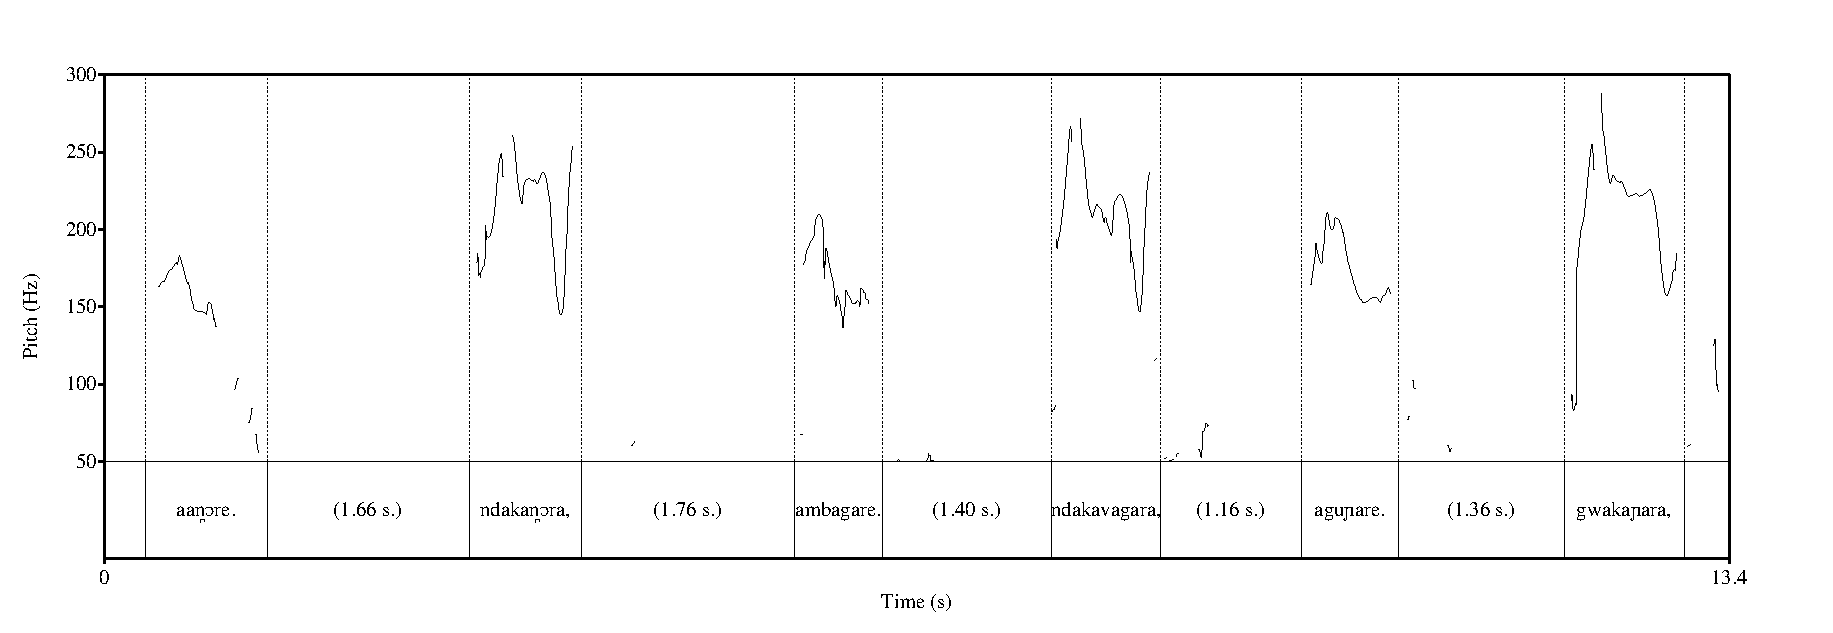
\includegraphics[width=4.8in]{figures/sarvasyFig1.eps}}
\caption{Intonation contour produced with PRAAT for six-clause reference-bridging sequence in (\ref{Saex:2ad}). \label{SaFig1}}
\end{figure}

Thus, \ili{Logoori} bridging clauses are both morphologically \isi{finite} and prosodically dependent, as in \ili{Oceanic} languages and \ili{Jingulu} (Australia; see \chapref{ch:1}, this volume).

\subsection{Logoori bridging construction semantics}
\label{Sasemantics}
Semantically, \ili{Logoori} bridging clauses in these two \isi{procedural texts} uniformly accompany temporal \isi{sequentiality}: the bridging clause makes it clear that the \isi{action} described in the succeeding clause (the clause after the bridging clause) temporally follows the \isi{action} described in the reference clause. This is facilitated by the omnipresence of the Immediate Perfect inflection, meaning ``once X has V-ed...'' or ``X having just V-ed...'' in the bridging clause. Beyond simple \isi{sequentiality}, the semantics of the Immediate Perfect inflection also mean that there is a close temporal connection between the two actions: they are never distant in time.

The characteristics of \ili{Logoori} recapitulative bridging constructions in \isi{procedural texts} are summarized in Table \ref{SaTabl1}.



% Please add the following required packages to your document preamble:
% \usepackage{multirow}

% \begin{table}[]
% \small
% \caption{Characteristics of bridging constructions in Logoori procedural texts}
% \label{SaTabl1}
% \begin{tabular}{lll}
% \lsptoprule
%                                     & \textbf{Reference clause} & \textbf{Bridging clause}       \\
% \midrule
% \multirow{2}{*}{\textbf{Tense}}     & Narrative, or             & Immediate Perfect              \\
%                                     & periphrastic Near Future  &                                \\    \cline{1-3}
%                                      &                      &                       \\ 
% \textbf{Subject person\slash number}      & Free                      & As in the reference clause     \\ \cline{1-3}
%                                     &                      &                       \\                 
% \multirow{5}{*}{\textbf{Semantics}} &    						  & Close temporal link between      \\
%                                     & Introduction of                    & \isi{action} in the reference  \\
%                                     & a new \isi{action}                           & clause and \isi{action} in the    \\
%                                     &                           & succeeding clause                        \\ \cline{1-3}
%                                       &                      &                       \\                                   
%  \textbf{Prosody}                    & Final                     & Non-final                      \\
% \lspbottomrule
% \end{tabular}
% \end{table}


\begin{table}
\small
\caption{Characteristics of bridging constructions in Logoori procedural texts}
\label{SaTabl1}
\begin{tabularx}{\textwidth}{lQQ}
\lsptoprule
 & {Reference clause} & {Bridging clause}       \\
\midrule
{Tense}     & Narrative, or  periphrastic Near Future           & Immediate Perfect              \\ \tablevspace 
{Subject person\slash number}      & Free                      & As in the reference clause     \\ \tablevspace                 
{Semantics} &    	Introduction of a new \isi{action}  & Close temporal link between \isi{action} in the reference clause and \isi{action} in the succeeding clause\\\tablevspace
{Prosody}                    & Final                     & Non-final                      \\
\lspbottomrule
\end{tabularx}
\end{table}

\subsection{Marginal bridging constructions}
\label{Samarginal}
One of the bridging clauses in \citet{Chesi2014}, and four potential bridging clauses identified in non-\isi{procedural texts} in the corpus, do not follow the pattern in (\ref{Saex:2ad}) and (\ref{Saex:6ab}). These clauses feature lexical \isi{repetition} in the predicate from a previous clause, but it is unclear whether they should be considered bridging clauses. 

For instance, the corpus includes another text by Mbone describing how\linebreak women used to live in the olden days. The potential bridging clause occurs in the sequence given in (\ref{Saex:7ac}). Here, the inflected Far Past tense verb \textit{va-a-ragel-a} `they used to eat \textit{vuchima}' occurs near the end of the first \isi{prosodic} sentence and also begins (in identical inflection) the second sentence. 
 
\begin{exe}
\ex \label{Saex:7ac}
\begin{xlist}
\ex \label{Saex:7a}
\gll Kaande,  kare,  va-kere   va-a-r-aŋge     ne   zi-sahane  zja   va-a-ragel-a       ko   daave. \\
again    old  \textsc{2}-woman  \textsc{2}-\textsc{fp}-exist-\textsc{progr}  with  \textsc{10}-plate  \textsc{10}.\textsc{rel}  \textsc{2}-\textsc{fp}-squeeze.\textit{vuchima}-\textsc{fv}  \textsc{loc}  \textsc{neg}\\
\glt \sqt{Again, in olden days, women did not have plates on which they used to squeeze \textit{vuchima.}}\\
\ex \label{Saex:7b}
\gll Va-a-ragel-a,       vi-ndo   vja   va-a-raŋg-a,  ri-dero,  \\
   \textsc{2}-\textsc{fp}-squeeze.\textit{vuchima}-\textsc{fv} \textsc{8}-thing  \textsc{8}.\textsc{rel}  \textsc{2}-\textsc{fp-}call-\textsc{fv}  \textsc{5}-\textit{dero}  \\
   \glt \sqt{They used to squeeze \textit{vuchima} (on), things that they called \textit{ridero},} \\
\ex \label{Saex:7c}
\gll vijo   vja   va-a-ragel-a,       kaande...\\     	       
    \textsc{8}.\textsc{dem}  \textsc{8}.\textsc{rel}  \textsc{2}-\textsc{fp}-squeeze.\textit{vuchima}-\textsc{fv}  again\\
\glt \sqt{it was (on) those that they used to squeeze \textit{vuchima}, again...} 
\end{xlist}
\end{exe}



The first clause in (\ref{Saex:7b}) could be considered a bridging clause since the last verb in (\ref{Saex:7a}), \textit{va-a-ragel-a}, is repeated there. This would be similar to the bridging constructions in \refsec{Sa21form} in that the lexical verb root and subject person\slash number are the same in the reference clause and the (possible) bridging clause. But unlike the true bridging constructions introduced earlier, the recapitulation in the first clause of (\ref{Saex:7b}) also has the same tense as the earlier instance: in fact, the form is exactly the same. In this case, since \textit{va-a-ragel-a} is also repeated a second time later in (\ref{Saex:7c}), its \isi{repetition} at the beginning of (\ref{Saex:7b}) may be interpretable as not a bridging clause, but simply as expansion of the theme in (\ref{Saex:7a}), which then continues throughout. 

Two other instances of lexical \isi{repetition} that diverge from the bridging construction pattern in \refsec{Sa21form} come from a fairy tale told by Ms. Grace Otieno. Here, two clauses that begin new \isi{prosodic} sentences feature lexical \isi{repetition} of predicates from the preceding sentences. But in both cases, the word \textit{ruwa} `while, when' precedes the recapitulated verb. This would seem to be a different type of linkage than the simple recapitulation in \refsec{Sa21form}. One of these examples is in (\ref{Saex:8ab}):
 
\begin{exe}
\ex \label{Saex:8ab}
\begin{xlist}
\ex \label{Saex:8a}
\gll ...ne  ji-i-ran-a  je-eŋgo. \\
and  \textsc{1}-\textsc{fp}-return-\textsc{fv}  \textsc{1}-home\\
\glt \sqt{...and he returned to his home.}\\
\ex \label{Saex:8b}
\gll Ruwa  ji-i-ran-a,  ja-a-n̪ɔr-a...\\     	       
   when  \textsc{1-fp}-return-\textsc{fv}  \textsc{1-fp}-find-\textsc{fv}\\
\glt \sqt{When he returned, he found...} 
\end{xlist}
\end{exe}

Such examples are included in parentheses in the final counts of bridging constructions in Table \ref{SaTabl2}, in the last section \refsec{Saconcl}. Similarly, the only potential bridging clause in \citet{Chesi2014} that does not follow the pattern in \refsec{Sa21form} may serve a different function from the bridging clauses there. This is seen in example (\ref{Saex:9ab}) below:

\begin{exe}
\ex \label{Saex:9ab}
\begin{xlist}
\ex \label{Saex:9a}
\gll ...ko-taŋg-e ko-raag-ir-a. Na-vo. \\
\textsc{1pl}-begin-\textsc{fv} \textsc{15}-squeeze.\textit{vuchima}-\textsc{appl-fv} \textsc{comit-2}\\
\glt \sqt{...We (will) start to squeeze \textit{vuchima}. With them.}\\
\ex \label{Saex:9b}
\gll Ko-taŋg-e ko-raag-ir-a nɛɛndɛ va-geni va-aŋge...\\     	       
   \textsc{1pl-}begin-\textsc{fv} \textsc{15}-squeeze.\textit{vuchima}-\textsc{appl-fv} \textsc{comit} \textsc{2}-guest \textsc{2}-\textsc{1sg.poss}\\
\glt \sqt{We (will) start to squeeze \textit{vuchima} along with my guests...} 
\end{xlist}
\end{exe}


Here, the speaker originally simply states in (\ref{Saex:9a}) that ``we (will) begin to squeeze \textit{vuchima}'', without indicating who are included in ``we''. She begins to expand on this with the explanatory fragment \textit{na-vo} `with them', but explains even more precisely in (\ref{Saex:9b}). This explanation includes a verbatim \isi{repetition} of the phrase ``we (will) begin to squeeze \textit{vuchima}''. But this \isi{repetition} arguably functions more to explain and expand on the earlier instance than to foster discourse coherence; it is thus considered only marginal bridging here.


\section{Alternatives to bridging clauses: nominal repetition}
\label{Saalternatives}
Most of the \ili{Logoori} corpus examined is remarkably free of bridging constructions or any other \isi{repetition} of verbal predicates (numbers are given in Table \ref{SaTabl2} in the last section, \refsec{Saconcl}). In the \ili{Logoori} texts that are organized thematically \citep{farr99}, there is a different type of lexical \isi{repetition}. Here, the final NP of a preceding \isi{prosodic} sentence sometimes recurs in the beginning of the following sentence. This may be natural for languages with AVO constituent order; the O argument of the preceding clause can be the subject of the following clause. An example from a Grace Otieno text on games played in the olden days is in (\ref{Saex:10ab}):


\begin{exe}
\ex \label{Saex:10ab}
\begin{xlist}
\ex \label{Saex:10a}
\gll Mu-keno  gw-oonde  gw-a-raŋg-w-a    zi-seembe. \\
\textsc{3}-game    \textsc{3}-other    \textsc{3}-\textsc{fp}-call-\textsc{pass}-\textsc{fv}  \textsc{10}-\textit{seembe}\\
\glt \sqt{Another game was called \textit{ziseembe}.}\\
\ex \label{Saex:10b}
\gll Zi-seembe  zj-a-kob-aŋg-w-a    hari  ka-ɲiŋge.\\     	       
   \textsc{10}-\textit{seembe}  \textsc{10}-\textsc{fp}-play-\textsc{progr}-\textsc{pass}-\textsc{fv}  time  \textsc{12}-many\\
\glt \sqt{\textit{Ziseembe} used to be played many times.} 
\end{xlist}
\end{exe}


This sort of \isi{repetition} could be considered a type of bridging involving \isi{NPs} rather than verbal predicates. While bridging clauses promote event continuity in discourse, bridging \isi{NPs} arguably maintain discourse coherence relating to \isi{NPs}. 

There is no apparent discourse context where bridging \isi{NPs} are requisite. A common context is that of (\ref{Saex:10ab}), where something is introduced at the end of one sentence and reiterated at the beginning of the second sentence. Another example is in (\ref{Saex:11ab}), from a text by Mr. Benjamin Egadwe on the benefits of bovine husbandry:


\begin{exe}
\ex \label{Saex:11ab}
\begin{xlist}
\ex \label{Saex:11a}
\gll ...no  o-ɲor-a   mo   zi-seendi. \\
 \textsc{conj}  \textsc{2sg}-find-\textsc{fv}  \textsc{loc}  \textsc{10}-money\\
\glt \sqt{...and you find in it money.}\\
\ex \label{Saex:11b}
\gll Zi-seendi   zi-ra,     zi-ra-ko-koɲ-a   ko...\\     	       
  \textsc{10}-money  \textsc{10}-\textsc{dem}  \textsc{10}-\textsc{nf-2pl-}help-\textsc{fv}  with\\
\glt \sqt{That money, it will help you with...} 
\end{xlist}
\end{exe}


Not counted as ``bridging \isi{NPs}'' here are lexical repetitions from earlier parts of preceding sentences. In some instances, such \isi{repetition} features the same lexical root but a different noun class marker, as in the consecutive sentence fragments in (\ref{Saex:12ab}), from a descriptive text by Grace Otieno on children’s games of yore: 


\begin{exe}
\ex \label{Saex:12ab}
\begin{xlist}
\ex \label{Saex:12a}
\gll ...neva  mi-keno   ʤe   ke-mwaamo  ʤe-n̪ar-a ko-taŋg-iz-w-a     mo   zi-skuru. \\
 if  \textsc{4}-game    \textsc{4}.\textsc{gen}  \textsc{7}-black    \textsc{4}-be.able-\textsc{fv}  \textsc{15}-begin-\textsc{appl}-\textsc{pass}-\textsc{fv}    \textsc{loc}  \textsc{10}-school\\
\glt \sqt{...if games of Africans can be introduced to schools.}\\
\ex \label{Saex:12b}
\gll Vu-keno   kore,  sugudi,   eŋgɔjɔ...\\     	       
  \textsc{14}-game  like  \textit{sugudi}    \textit{eŋgɔjɔ}\\
\glt \sqt{Play like \textit{sugudi}, \textit{eŋgɔjɔ}...} 
\end{xlist}
\end{exe}


Here, \textit{mi-keno} `games' and \textit{vu-keno} `play' share a lexical root but differ in noun class, as seen in the noun class prefix: Class 4, indicated with \textit{mi-}  here, is the usual plural of Class 3 nouns such as \textit{mu-keno} `game' in (\ref{Saex:10a}). The \textit{vu-} class, Class 14, includes some abstract conceptual nouns and some other collective nouns. While all lexical \isi{repetition} surely enhances discourse coherence, \isi{NPs} such as \textit{vu-keno} in (\ref{Saex:12b}) are not considered bridging \isi{NPs} here, since the reference NP occurs much earlier in the preceding sentence.

Rampant in \ili{Logoori} discourse, and much more widespread than bridging constructions involving either verbs or \isi{NPs}, are anaphoric demonstratives that promote discourse coherence across clauses in terms of reference. Three different noun-modifying demonstratives ``this'' and ``that'' encode three relational distances between speaker and the referent. These take the form of suffixes (or roots, depending on the analysis) to which noun class prefixes are added, as seen in examples (\ref{Saex:7c}) and (\ref{Saex:11b}). In addition to these, there is a fourth nominal modifier usually translated ``(that) particular'' by Mr. Indire that modifies elements that have been previously introduced. At least one adverbial demonstrative \textit{ndijo} `like that' is also used. Counts of all of these are given in Table \ref{SaTabl2} in the next section.
%
\section{Conclusion}
\label{Saconcl}
A summary of bridging and related construction counts in the small corpus consulted for this chapter is in Table \ref{SaTabl2}. ``Corpus 1'' refers to the Diercks corpus, ``corpus 2'' to texts recorded in the UCLA Field Methods class, and ``corpus 3'' to excerpts from the film Maragoli \citep{Nichols1976}.



\begin{sidewaystable}[]
\small
\caption{Summary of bridging-related constructions in Logoori sample corpus\todo[inline]{TODO}}
\label{SaTabl2}
\begin{tabular}{llclccrcd{2}}
\lsptoprule
{Text name}  & {Speaker} & {Corpus} & {Genre} & {Bridging } & {Bridging}     & \multicolumn{1}{c}{Nominal} & {Adverbial} & \textbf{Length}  \\
{}                  & {}        & {}       & {}      & {NP}            & {construction} & \multicolumn{1}{c}{anaphor} & {anaphor}   & \textbf{in min.} \\
\midrule
Games for children         & G. Otieno        & 1         & Descriptive    & 8                    & 0                     & 11               & 4                  & 7:51             \\
Old flour                  & L. Mbone        & 1         & Descriptive    & 0                    & (1)                   & 4                & 0                  & 2:04             \\
Girls who wanted luck      & G. Otieno        & 1         & Fairy tale     & 0                    & (2)                   & 11               & 3                  & 5:42             \\
Woman and the hen          & G. Otieno        & 1         & Fairy tale     & 0                    & 0                     & 5                & 3                  & 4:56             \\
On Murogooli              & S. Magono        & 1         & Narrative      & 2                    & 0                     & 4                & 1                  & 3:07             \\
How to care for cows       & B. Egadwe        & 1         & Descriptive    & 4                    & 0                     & 23               & 6                  & 5:47             \\
Preparing tea              & L. Mbone        & 1         & Process        & 0                    & 3                     & 2                & 0                  & 1:20             \\
Lunchtime food             & C. Chesi         & 1         & Process        & 0                    & 13 (1)                & 4                & 1                  & 2:42             \\
Childhood games            & M. Indire        & 2     & Descriptive    & 0                    & 0                     & 1                & 0                  & 0:52             \\
Future wishes              & M. Indire        & 2     & Narrative      & 0                    & 0                     & 1                & 0                  & 0:48             \\
Monkey and dog             & M. Indire        & 2     & Narrative      & 0                    & (1)                   & 1                & 1                  & 1:30             \\
Yesterday, today,  & M. Indire        & 2     & Narrative      & 0                    & 0                     & 0                & 0                  & 3:23             \\
and tomorrow &         &      &       &                     &                      &                 &                   &             \\
Women on barns   & various          & 3       & Conversation  & 1                    & 0                     & 0                & 0                  & 1:18             \\
 and hunger  &           &        &   &                     &                      &                 &                   &           \\
Men on many children       & various          & 3      & Descriptive    & 0                    & 0                     & 0                & 0                  & 0:28        \\  
\lspbottomrule  
\end{tabular}
\end{sidewaystable}
%

In Table \ref{SaTabl2}, counts for the marginal bridging constructions described in \refsec{Samarginal} are given in parentheses.\todo{Move this sentence to the caption?}  
 
Table \ref{SaTabl2} shows that of the narratives and conversations sampled, only two have more than one non-marginal bridging construction involving verbs. Both of these are procedural descriptions. But these procedural descriptions differ in degree to which they employ recapitulative constructions. As seen in Table \ref{SaTabl2}, ``bridging \isi{NPs}'' -- \isi{NPs} that employ lexical \isi{repetition} with the effect of correlating a preceding sentence with the following one -- occur in three of the texts that lack verb-based bridging constructions entirely. But by far the most common device to link concepts in a sentence to earlier sentences is use of anaphors, either NP modifiers or predicate anaphors. 

\citeauthor{guerin18} (\chapref{ch:1}, this volume) define recapitulative bridging as involving clauses -- a reference and a bridging clause, and, by implication, a clause after the bridging clause that might be called the ``succeeding'' clause. In the small corpus consulted for this chapter, \ili{Logoori} recapitulative bridging is highly genre-specific, limited to \isi{procedural texts}. Even within these texts, recapitulative bridging has uneven distribution. Although both \isi{procedural texts} include them, this is in greatly differing proportions -- even across two different sections of the same text -- so there seems to be no genre-related requirement of bridging. The two texts also differ in that \citet{Mbone2014} uses a kind of abridged bridge with no recapitulation: many of that speaker’s independent clauses feature the same inflection as bridging clauses, seemingly eliminating the need for bridging.

\ili{Logoori} recapitulative bridging constructions seem to scaffold a tightly \isi{sequential} interpretation of actions. As anticipated by \citeauthor{guerin18} (\chapref{ch:1}, this volume), the discourse units in \ili{Logoori} \isi{procedural texts} are short; the bridging clause serves as a bridge between single-clause units. 

Another type of recapitulation that arguably serves to bridge two sentences involves ``bridging \isi{NPs}'' rather than clauses. In the \ili{Logoori} corpus here, recapitulation in the vessel of \isi{NPs} uniformly occurs in descriptive texts, where concepts, rather than actions or events, are central. But both bridging \isi{NPs} and bridging clauses are largely absent from narratives, where \ili{Logoori} speakers seem to prefer a streamlined, non-repetitive discourse flow. \citet{seifart10} argued that bridging in \ili{Bora} occurs in the form of pronouns because of the prevalence of \isi{NPs} over predicates in \ili{Bora} discourse. While \citet{seifart10} justifies the use of ``bridging pronouns'' in \ili{Bora} through a general preference that supercedes discourse genre, in \ili{Logoori} it is apparently the \isi{text genre} that determines which type of recapitulation -- predicative or NP -- is primary in promoting discourse coherence.

The absence of bridging constructions from most of the \ili{Logoori} corpus sampled here shows that \isi{clause chaining} and agglutinative, complex verbal morphology are not necessarily conducive to bridging construction use in discourse. Since recapitulative bridging constructions are present in some parts of the corpus, however, there is no structural incompatibility with their use. Mbone’s application of the Immediate Perfect inflection for a similar effect to recapitulative bridging hints at a possible factor in their absence from most of the corpus: the rich \ili{Logoori} inventory of highly-specific \isi{TAM} inflections. This could combine with a possible stylistic dispreference for recapitulation by \ili{Logoori} orators to limit use of bridging constructions, either nominal or clausal.


\section*{Appendix}
\setcounter{equation}{0}
\exewidth{(A23)}
The text here is excerpted from a \isi{procedural text} recorded by Ms. Carolyn Chesi in 2014 as part of the \ili{Logoori} corpus commissioned by Michael Diercks.


 \begin{exe}
\exi{(A1)} \label{Saapp1}
\gll Ko-meet-a va-naaŋg-a, Kaarɔlini, ʧeesi,\\     	       
\textsc{15}-start-\textsc{fv}  \textsc{2}-\textsc{1sg}.call.\textsc{progr}-\textsc{fv}  Carolyn  Chesi \\
\glt \sqt{To begin [n.d., idiomatic] they call me Carolyn, Chesi, } 
\end{exe}

 \begin{exe}
\exi{(A2)} \label{Saapp2}
\gll na-n̪en̪-aa, n-zah-e, o-mo-tera, gwa-aŋge,\\
\textsc{narr}-\textsc{1sg}.want-\textsc{pres}.\textsc{fv}  \textsc{1sg}-uproot-\textsc{fv}  \textsc{pre}-\textsc{3}-\textit{tera}  \textsc{3}-\textsc{1sg}.\textsc{poss}\\
\glt \sqt{and I want to uproot my \textit{mutere},}
\end{exe}

 \begin{exe}
\exi{(A3)} \label{Saapp3}
\gll gwa man̪-e n-dug-er-e, lanstaim.\\
\textsc{3}.\textsc{rel}  \textsc{1sg}.want-\textsc{fv}  \textsc{1sg}-prepare.cornmeal-\textsc{appl}-\textsc{fv}  lunchtime\\
\glt \sqt{which I will prepare, at ``lunchtime''.}
\end{exe}

 \begin{exe}
\exi{(A4)} \label{Saapp4}
\gll Man̪-a n-zj-e m̩-mo-rɛmɛ,\\
\textsc{1sg}.want-\textsc{fv}   \textsc{1sg}-go-\textsc{fv}   \textsc{loc}-\textsc{3}-land\\
\glt \sqt{I will go to the farm,}
\end{exe}

 \begin{exe}
\exi{(A5)} \label{Saapp5}
\gll n-zj-e kw-ah-a i-ri-kove,\\
\textsc{1sg}-go-\textsc{fv}   \textsc{15}-uproot-\textsc{fv}   \textsc{pre}-\textsc{5}-\textit{kove}\\
\glt \sqt{I go uproot \textit{rikove}, [n.d., green ``cowpea leaves'']}
\end{exe}

 \begin{exe}
\exi{(A6)} \label{Saapp6}
\gll aa-n-zah-e nɛɛndɛ mo-tere,\\
\textsc{narr}-\textsc{1sg}-uproot-fv   \textsc{comit}   \textsc{3}-\textit{tera}\\
\glt \sqt{I uproot it along with \textit{omotera},}
\end{exe}

 \begin{exe}
\exi{(A7)} \label{Saapp7}
\gll \underline{\smash{aa-n̪ɔr-e}}.\\
\textsc{narr-1sg.}pick.leaves.from.stems\textsc{-fv}\\
\glt \sqt{I pick the leaves from the stems.}
\end{exe}

 \begin{exe}
\exi{(A8)} \label{Saapp8}
\gll \textbf{N-daka-n̪ɔr-a},          \underline{\smash{a-m-bagar-e}}.\\
\textsc{1sg}-\textsc{imm.pf-}pick.leaves.from.stems-\textsc{fv}  \textsc{narr-1sg}-lay.out.to.dry-\textsc{fv}\\
\glt \sqt{Once I have picked the leaves from the stems, I lay them out to dry.}
\end{exe}

 \begin{exe}
\exi{(A9)} \label{Saapp9}
\gll \textbf{N-daka-vagar-a},      \underline{\smash{a-gu-ɲar-e}}.\\
\textsc{1sg-imm.pf-}lay.out.to.dry-\textsc{fv}  \textsc{narr-3}-shrivel-\textsc{fv}\\
\glt \sqt{Once I have laid them out to dry, they shrivel.}
\end{exe}

 \begin{exe}
\exi{(A10)} \label{Saapp10}
\gll \textbf{Gw-aka-ɲar-a},\\
\textsc{3}-\textsc{imm.pf-}shrivel-\textsc{fv}\\
\glt \sqt{They having shriveled,}
\end{exe}

 \begin{exe}
\exi{(A11)} \label{Saapp11}
\gll e-man̪-a e-dook-e e-saa,\\
\textsc{9}-want-\textsc{fv}  \textsc{9}-arrive-\textsc{fv}  \textsc{9}-hour\\
\glt \sqt{it will arrive at the hour,}
\end{exe}

 \begin{exe}
\exi{(A12)} \label{Saapp12}
\gll ʃímbe saa tanɔ,\\
about \textsc{9}.hour  five\\
\glt \sqt{near eleven o'clock,}
\end{exe}

 \begin{exe}
\exi{(A13)} \label{Saapp13}
\gll saa siita,  \underline{a-m-bek-e} \underline{ko} \underline{\smash{ma-higa}}.\\
\textsc{9}.hour  six  \textsc{narr}-\textsc{1sg}-put-\textsc{fv}  \textsc{loc} \textsc{6}-stove\\
\glt \sqt{twelve o'clock, then I will put (it) on the stove.}
\end{exe}

 \begin{exe}
\exi{(A14)} \label{Saapp14}
\gll \textbf{N-daka-vek-a} \textbf{ko} \textbf{ma-higa},\\
\textsc{1sg-imm}.\textsc{perf}-put-\textsc{fv}  \textsc{loc}  \textsc{6}-stove\\
\glt \sqt{Once I have put it on the stove,}
\end{exe}

 \begin{exe}
\exi{(A15)} \label{Saapp15}
\gll \underline{na} \underline{\smash{ŋ-gerek-el-a}} \underline{\smash{muɲu}}.\\
then  \textsc{1sg}-leach-\textsc{appl}-\textsc{fv} \textsc{3}.soup\\
\glt \sqt{then I leach soup.}
\end{exe}

 \begin{exe}
\exi{(A16)} \label{Saapp16}
\gll \textbf{N-daka-mor-a} \textbf{gw-a-kerek-el-a} \textbf{muɲu},\\
\textsc{1sg}-\textsc{imm.pf}-finish-\textsc{fv} \textsc{3}-\textsc{past}?-leach-\textsc{appl}-\textsc{fv}  \textsc{3}.soup  \\
\glt \sqt{Once I have leached soup,}
\end{exe}

 \begin{exe}
\exi{(A17)} \label{Saapp17}
\gll man̪-a m-bogor-e n-zog-iz-e,\\
\textsc{1sg}.want-\textsc{fv}  \textsc{1sg}-take-\textsc{fv}  \textsc{1sg}-wash-\textsc{appl}-\textsc{fv}\\
\glt \sqt{I will take it and wash it,}
\end{exe}

 \begin{exe}
\exi{(A18)} \label{Saapp18}
\gll a-ŋ-gamor-e,\\
\textsc{narr}-\textsc{1sg}-wring-\textsc{fv}\\
\glt \sqt{then I will wring it,}
\end{exe}

 \begin{exe}
\exi{(A19)} \label{Saapp19}
\gll a-m-bogor-e muɲu m-bek-e mu i-ɲiŋgu,\\
\textsc{narr}-\textsc{1sg}-take-\textsc{fv}  \textsc{3}.soup    \textsc{1sg}-put-\textsc{fv}  \textsc{loc}  \textsc{9}-earthen.pot\\
\glt \sqt{I will take the soup and put it in an earthen pot,}
\end{exe}

 \begin{exe}
\exi{(A20)} \label{Saapp20}
\gll a-m-bek-e m̩ to-ze ki-dɔɔkɔ.\\
\textsc{narr}-\textsc{1sg}-put  \textsc{loc}  \textsc{13}-water  \textsc{7}-little\\
\glt \sqt{then I will put in it a little water a bit.}
\end{exe}

 \begin{exe}
\exi{(A21)} \label{Saapp21}
\gll A-m-bek-e ko ma-ʃiga.\\
\textsc{narr}-\textsc{1sg}-put-\textsc{fv}  \textsc{loc}  \textsc{6}-stove\\
\glt \sqt{And I will put it on the stove.}
\end{exe}

 \begin{exe}
\exi{(A22)} \label{Saapp22}
\gll A-go-ʃj-e,\\
\textsc{narr}-\textsc{3}-cook-\textsc{fv}\\
\glt \sqt{It will cook,}
\end{exe}

 \begin{exe}
\exi{(A23)} \label{Saapp23}
\gll A-n-ʤokaɲ-e m̩.\\
\textsc{narr}-\textsc{1sg}-stir-\textsc{fv}  \textsc{loc}\\
\glt \sqt{then I stir in it.}
\end{exe}

\section*{Abbreviations}
\begin{multicols}{2}
\begin{tabbing}
\textsc{1sg, 2sg, 1pl}, etc. \hspace{.5em}  \= person\slash number\kill
\textsc{1sg, 2sg, 1pl}, etc.   \> person\slash number\\
\textsc{1, 2, 3, ..., 15}   \>   noun class\\
\textsc{appl}   \>   applicative\\
\textsc{conj}   \>   conjunction\\
\textsc{dem}    \>  demonstrative\\
\textsc{dep}    \>  dependent\\
\textsc{fp}     \>  far past\\
\textsc{fv}     \>  final vowel\\
\textsc{imm.pf} \>   immediate perfect\\
\textsc{loc}    \>   locative\\
\textsc{mv}     \> medial verb\\
\textsc{narr}   \>  narrative\\
\textsc{neg}    \>   negation\\
\textsc{nf}     \>  near future\\
\textsc{nsg}    \>  non-singular\\
\textsc{o}      \> object\\
\textsc{pass}   \>   passive\\
\textsc{poss}   \>    possessive\\
\textsc{pre}    \>   pre-prefix\\
\textsc{pres}   \>    present\\
\textsc{progr}  \>   progressive\\
\textsc{rel}    \>   relative\\
\textsc{rp}     \>  remote past\\
\end{tabbing}
\end{multicols}


\section*{Acknowledgements}
Many thanks to Mwabeni Indire, Michael Diercks, Sandra Nichols, the UCLA Field Methods PhD students, Valérie Guérin, two anonymous reviewers, and the speakers from Michael Diercks’s corpus. 

\sloppy

\printbibliography[heading=subbibliography,notkeyword=this] 
\end{document}
